% #!luajitlatex
\IfFileExists{luatex85.sty}{\RequirePackage{luatex85}}{}
\documentclass{ltjsarticle}
\usepackage{mystyle}
\title{\TeX~Liveのインストール}
\hypersetup{pdftitle={TeX Liveのインストール}}
\captionsetup{justification=centering, labelfont={small, rm}}

\makeatletter
\def\UPDTIME{%
  \expandafter\@UPD@a\romannumeral-`0\pdfcreationdate!}
\def\@UPD@a#1#2#3#4#5#6{% Year
  #3#4#5#6/\@UPD@b}
\def\@UPD@b#1#2#3#4#5#6#7#8{% Month, Day, Hour, Min
  #1#2/#3#4~#5#6:#7#8:\@UPD@c
}
\def\@UPD@c#1#2#3!{% Sec
  #1#2}
\makeatother

\begin{document}
\baselineskip1.75\zw
\maketitle

\TeX はDonald~E. Knuth氏による「(特にたくさんの数式を含んだ)文書を
製作するためのシステム」である.
投稿を\TeX 形式のファイル(\TeX ソース)で受け付ける論文誌も多く,
数学・情報科学などの理工系では必須のソフトウェアといえる.
\medskip

実際には,Leslie Lamport氏による\TeX 上のマクロパッケージ\emph{\LaTeX}を使うことが多い.
\TeX は,「テフ」「テック」などと,\LaTeX は「ラテフ」「ラテック」「レイテック」などと読ば
れる.テキストでは,\TeX,~\LaTeX はそれぞれ\texttt{TeX},~\texttt{LaTeX}と表記されることに
なっている.


\medskip
本実習では,まず\TeX システムを実習用マシンにインストールすることからはじめる.
Windowsでの\TeX システムとしては,昔から角藤亮氏による
\href{http://w32tex.org/index-ja.html}{W32\TeX}が主流であったが,
本実習では\href{http://www.tug.org/texlive/}{\emph{\TeX~Live~2016}}%
を用いることにする\footnote{%
  \href{http://www.tug.org/texlive/}{\emph{\TeX~Live}}%
  は,世界中の\TeX に関するプログラム・パッケージ類を収めたものであり,
  毎年一回リリースされている.日本語対応も近年(2010--2013年)強化されており,
  まともに扱えるものになってきた.
  %%% たぶん実習時点ではこうなってるはず
  % なお,\TeX~Live~2013の更新は4月初旬で終了しており,
  % 現在はTL~2014 pretestが行われている段階である.
}.

\medskip
\TeX~Liveをインストールした後は,各自の知識に沿って実習を進めてほしい,
計算数学実習資料集の
「\href{http://material.utmsks.net/home/platex2017}{\TeX 実習(2017)}」
%%% まだ作ってない
のページ内にある「\TeX 実習」を参照すること.

\medskip
以下,\url{about:blank}のような部分は外部リンクで,
緑字の部分は文書内リンクである.

\vfill

{\scriptsize\raggedleft
  Last update: {\tt\UPDTIME}.
  \par}


\newpage

\setcounter{section}{-1}

\section{はじめに}
本実習では,
奥村晴彦/黒木裕介著「\LaTeXe 美文書作成入門 改訂第7版」
の付属の DVD (の中身)を用いて \TeX~Live のインストールを行う.

まずはインストール前の準備をしよう.

\begin{enumerate}
  \itemsep\medskipamount
  \setcounter{enumi}{-1}
\item コントロールパネル\footnote{左下の Windows ボタンを右クリックすると一覧に出てくる}
  右上の検索ボックスに「拡張子」と入力して検索し,
  「ファイルの拡張子の表示または非表示」を選択.
  現れた画面下部の「詳細設定」をスクロールし,
  下の方にある「登録されている拡張子は表示しない」のチェックを\emph{外す}.

  \begin{itemize}
  \item \TeX 実習に限らず,本授業の実習ではこの設定にしておいた方が良い.
  \item 「拡張子」やこの設定の意味が分からない場合は,
    インターネットで検索するか TA に聞くなどして,今のうちに理解しておくと良いだろう.
  \end{itemize}
\item Windows~10のインストールに使用したUSBメモリから,
  \TeX~Liveのインストーラ(USBメモリ内の\texttt{tex¥}%
  \hskip\ltjgetparameter{xkanjiskip}以下全体)を
  デスクトップ以下にコピーする.
  \begin{itemize}
  \item USB 3.0 (青い USB 端子) に挿した方が速く,2分程度で終了する.
  \item コピーし終わった後は,USBメモリはもう必要ない.
  \end{itemize}
\item \texttt{tex} ディレクトリの中には,
  \texttt{win}と\texttt{mac},そして \texttt{texlive2016} の3つのディレクトリがある.
  本実習では,前者2つは使用せず,\texttt{texlive2016} の中身のみを使用する.
  \begin{itemize}
  \item 書籍では \texttt{tex¥win¥美文書TeXセットアップ.exe} の実行を推奨している.
    この方法であれば数回「次へ」をクリックするだけでインストールができるが,
    \TeX~Live をフルインストールすることになるため,多くの時間(30分)とディスク容量(5GB)がかかってしまう.
  \item 本実習では,ディスク容量は問題ないが時間を節約したいため,設定をカスタマイズしてインストールする.
  \item 受講生が自宅PCなどにインストールする場合は,基本的に書籍通りの方法で問題ないだろう.
  \end{itemize}
\end{enumerate}


\section{\TeX~Liveのインストール}
時間の都合で設定をカスタマイズしてインストールする.
時間(とディスク容量)に余裕があれば,このような複雑な設定をする必要はないことを注意しておく.
\begin{enumerate}
  \itemsep\medskipamount
  % \setcounter{enumi}{-1}
  % \item Windows~10のインストールに使用したUSBメモリから,
  %   \TeX~Liveのインストーラ(USBメモリ内の\texttt{tex¥}%
  %   \hskip\ltjgetparameter{xkanjiskip}以下全体)を
  %   デスクトップ以下にコピーする.

  %   \begin{itemize}
  % %   \item
  % %     USBのドライブレターはa,~cマシンでは\texttt{E},
  % %     bマシンでは\texttt{D}か\texttt{G}となるのが普通だが,場合によっては異なっているかもしれない.
  %   \item コピーし終わった後は,USBメモリはもう必要ない.
  %   \end{itemize}

\item 上でコピーしたものの中から \texttt{texlive2016¥} ディレクトリにある
  \texttt{install-tl\underline{-advanced}.bat}を
  「管理者として実行」する\footnote{%
    batファイルを右クリックすると「管理者として実行」という
    項目が出てきます.
  }\footnote{%
    USBメモリ内から直に実行しても良いが,
    20分程度かかってしまう(一方,一旦インストーラごとコピーしてからだと
    高々10分)ようである.
  }.
  % \begin{itemize}
  % \item 管理者権限を求められたら,
  %   TAを呼んでパスワードを入力してもらう.
  % \item 「\texttt{perl}が見つからない」などと言われ,
  %   インストーラが正しく起動できない場合は,
  %   ひとまず同じ班の他のUSBメモリに差し替えてもう一度同じ事を試すこと.
  % \end{itemize}
  \smallskip
  バックグラウンドでコマンドプロンプトのウィンドウが表示されるが,
  無視すること.

\item 「導入作業中はウィルス検知器を無効にするのが最善です.」
  というダイアログが出るが,無視して×をクリックして閉じる.
  「続行」を押しても閉じるようである..

\item \TeX~Liveは標準ではフルインストールする設定になっている.
  ディスク容量的にはあまり問題はないが,
  今回はインストール時間を減らすために次の設定を行なう.

  まず,インストーラの一番上にある
  「{選択したスキーム}」の右の「変更」をクリックし,
  % 図\nobreak\ref{sch}のように
  「{teTeXスキーム}」を選択
  \footnote{%
    ちなみに,\href{http://www.tug.org/tetex/}{te\TeX}というのは,
    Thomas Esser氏がメンテナンスをしていた,UNIX系OSのための\TeX システムである.
    以前は広く用いられてきたが,2006年に更新停止となった.
  },「OK」.
  % \begin{figure}[!h]
  %   \centering
  %   \includegraphics[scale=.6]{tl15scheme.png}
  %   \caption{スキーム選択画面}\label{sch}
  % \end{figure}

\item 下半分の「オプション」のうち,
  「font と macro のソースツリーを導入」を「いいえ」に,
  「TeX worksフロントエンドを導入」を「はい」に変更する.
  % インストーラ(図\nobreak\ref{top})下半分の「オプション」を,
  % 図\nobreak\ref{top}に示されているように,
  % \begin{itemize}
  % \item 「font と macro のソースツリーを導入」を「いいえ」に,
  % \item 「全ユーザ用に導入」を「はい」に,
  % \item 「\TeX works フロントエンドを導入」を「いいえ」に,
  %   % \item 「After installation $\ldots$」を「いいえ」に
  % \end{itemize}
  % 変更する.
  % (一部の項目は,デフォルトで上記の設定になっているかもしれない)

  % \clearpage
\item 上から2番目の「導入対象コレクション」の右の「変更」をクリックし,
  図\nobreak\ref{col}のように変更して,「OK」.
  図中では,チェックを外すものは青囲み,入れるものは赤囲みしてある.\\
  \emph{「日本語」のところにチェックが入っていることを確認すること.}

\item インストールを開始する前に,
インストーラ画面上部の「必要ディスク領域」が 2029MB
\footnote{操作手順によっては2015MB となる場合もあるが,おそらく問題ないだろう.}
となっていることを確認(図\nobreak\ref{top}).
もし違っていた場合は,これまでの設定を見直そう.

\item 最後に,インストーラ最下部の
  「\TeX\ Liveの導入」をクリックし,インストールを開始する.
  \begin{itemize}
  \item 正しく設定できていれば10分程で終了する.
  \item 所々動作が停止したように見えたり,「応答なし」と表示されたりするが,気にしない.
    長いとそのような状態が1分程度続くこともある.
    それ以上長く続いた場合はTAを呼ぶこと.
  \item 「導入プロセス」ウィンドウに「\TeX\ Live へようこそ!」と
    表示されたら完了.コマンドプロンプトも一緒に閉じておくこと.
  \end{itemize}

  \clearpage
  \begin{figure}[t]
    \centering
    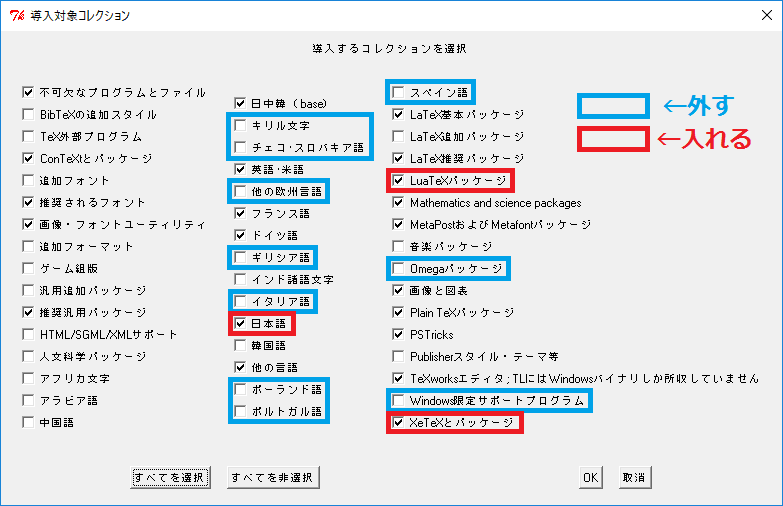
\includegraphics[scale=.7]{tl16col.png}
    \caption{コレクション選択画面}\label{col}
  \end{figure}

  \begin{figure}[b]
    \centering
    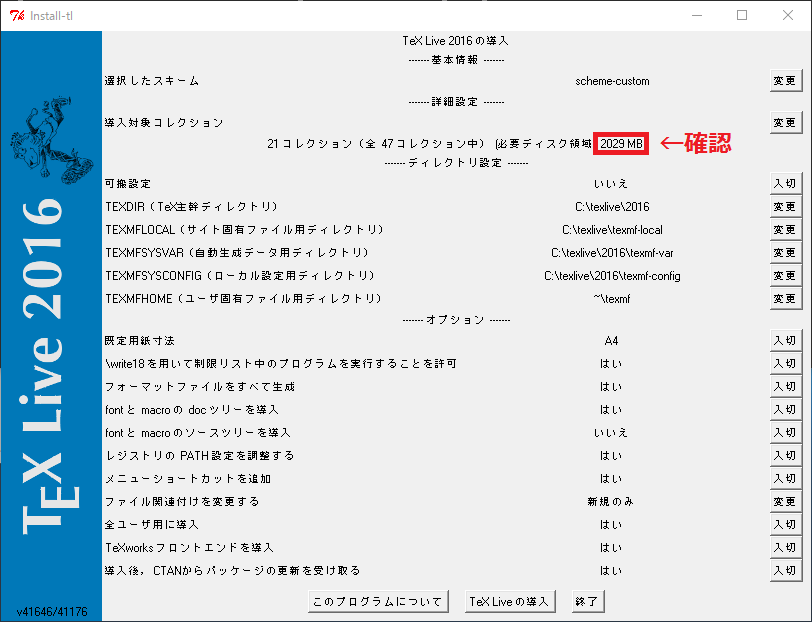
\includegraphics[scale=.5]{tl16top.png}
    \caption{インストーラ画面}\label{top}
  \end{figure}
\end{enumerate}


% \newpage
\section{EmEditor~Freeのインストール}
\TeX ソースを記述するにはメモ帳でもできないことはないが,
それよりは高機能なテキストエディタを用いるのが便利である.
\emph{自分で使い慣れたエディタ(\TeX works, Emacs, Vim等)が
  既にあればそれを使えばよい}が,
ここでは例として\emph{EmEditor Free}のインストールを述べる.

ちなみに,EmEditor Free で(拡張子が\texttt{.tex}となっている)\TeX ソースを開くと,
基本的なキーワードに色が付いて見易く表示される.

\begin{enumerate}
\item \emph{EmEditor}を
  \href{http://jp.emeditor.com/}{公式ページ}%
  の「今すぐダウンロード」からダウンロードする.% (図\nobreak\ref{emed1}).
  % \begin{figure}[!h]
  %   \centering
  %   \includegraphics[scale=.36]{em01.png}
  %   \caption{}\label{emed1}
  % \end{figure}
\item ダウンロードしたファイル\footnote{2017/4/10時点では\texttt{emed64\_16.6.0.exe}であ
    る.}を実行し,インストールを開始する.
  \begin{itemize}
  \item 「インストールタイプ」は「すべてのユーザ」
  \item セットアップタイプは「標準」でよい.% (図\nobreak\ref{emed2}).
    % \item 管理者権限を求められたら、TAを呼んでパスワードを入力してもらう.
  \end{itemize}
  % \begin{figure}[!h]
  %   \centering
  %   \includegraphics[scale=.45]{em02.png}
  %   \caption{}\label{emed2}
  % \end{figure}
  % \clearpage

\item インストールが完了したら,EmEditorを起動する.
  % 図\nobreak\ref{emed3}のように,
  最終段階の画面で「EmEditor (64-bit)を起動する」にチェックを入れておけば,
  自動的に起動する.
  % \begin{figure}[!h]
  %   \centering
  %   \includegraphics[scale=.45]{em03.png}
  %   \caption{}\label{emed3}
  % \end{figure}

\item %EmEditorを起動したら,まず「更新オプション」(図\nobreak\ref{emed4})
  % というダイアログが表示される.この図のように,「更新を自動的にチェックしない」を選択し,「OK」.
  EmEditorを起動したら,% まず図\nobreak\ref{emed4}のようなダイアログが表示されるが,
  まず「自動更新チェックを有効にしますか?」と尋ねるダイアログが表示されるが,
  「更新をチェックしない」を選択する.
  % \begin{figure}[!h]
  %   \centering
  %   \includegraphics[scale=.45]{em04.png}
  %   \caption{}\label{emed4}
  % \end{figure}

  % \newpage
\item 「購入方法」というウィンドウが表示されるが,無視して「閉じる」.
\item この段階ではProfessional版を試用している状況なので,
  \emph{Free版にダウングレード}する.

  \begin{enumerate}
  \item % CtrlキーとQキーを同時に押し,
    % 図\nobreak\ref{emed5}の
    メニューバーの「ツール」から「クイック起動」を選択する.
  \item 左上の欄に「\texttt{ダウングレード}」と入力する.
  \item すると下部に「ダウングレード」という項目のみ表示されるので,
    そこを選択して「このコマンドを実行」.
  \item 「本当にEmEditor Freeにダウングレードしますか?」と聞いてくるので「はい」.
  \item EmEditor の再起動を要求されるので従う.
    % \begin{figure}[!h]
    %   \centering
    %   \includegraphics[scale=.45]{em05.png}
    %   \caption{}\label{emed5}
    % \end{figure}
  \end{enumerate}

\item 最後に,\emph{ファイルの関連付け}の設定を行う.
  ただし,以下の設定は \emph{\TeX~Live インストールが終了してから}行う\footnote{\TeX ソースとの関連付けは \TeX works と競合するため.}.
  \begin{enumerate}
  \item 「ツール」→「設定の関連付け」を選択する.% (図\nobreak\ref{emed6}).

    % \begin{figure}[!h]
    %   \centering
    %   \includegraphics[scale=.45]{em06.png}
    %   \caption{}\label{emed6}
    % \end{figure}

  \item 「設定の関連付け」ウィンドウの左下部の「EmEditorと関連付け」
    をクリックする.% (図\nobreak\ref{emed7}).
    % \begin{figure}[!h]
    %   \centering
    %   \includegraphics[scale=.45]{em07.png}
    %   \caption{}\label{emed7}
    % \end{figure}

    % \newpage
  \item 「EmEditorと関連付け」% (図\nobreak\ref{emed7p})
    の「拡張子」の列に\texttt{txt}があることを確認する.

  \item せっかくなので,\TeX ソースもEmEditorに関連付けてしまおう.
    「EmEditorと関連付け」ウィンドウの「追加」をクリックする.
    % \begin{figure}[!h]
    %   \centering
    %   \includegraphics[scale=.45]{em07p.png}
    %   \caption{}\label{emed7p}
    % \end{figure}

  \item 出てきたウィンドウ% (図\nobreak\ref{emed8})
    の「拡張子」の項目に\emph{半角小文字で}
    \texttt{tex}と入力.「ファイルの種類」「現在のアイコン」を適当に設定し,
    「OK」.
    % \begin{figure}[!h]
    %   \centering
    %   \includegraphics[scale=.45]{em08.png}
    %   \caption{}\label{emed8}
    % \end{figure}
    \begin{itemize}
    \item このとき「既に'TL.TeXworks.edit.2016'に関連付けられています」などのメッセージが出るが,
      気にせず「はい」を選択.
    \end{itemize}
  \end{enumerate}
\end{enumerate}
\end{document}
